% Teilauswertung 4
\newpage
\section{Lebenszeitmessung}
\label{sec:lebenszeit}
\paragraph{1)}\textbf{Single-Exponential Fit}\\
Zu Beginn der Auswertung wollen wir einen \enquote{Single-Exponential Fit} durch den Datensatz legen. Dieser Fit hat die Form:
\begin{gather}
    N(t) = N_0e^{-\frac{t}{\tau}}
\end{gather}
Wir wählen zum fitten eine Anfangszeit $t_{0}=\SI{5}{\nano\metre}$, um sicher zu sein, dass wir im exponentiellen Abschnitt er Daten befinden. Für die Anfangsintensität $N_0$ wählen wir denjenigen Wert der aufgenommenen Messreihe zur Anfangszeit $t_{0}$, also $N_0=N(t_{0})$, besitzt. Damit ergibt sich nur noch die Lebenszeit $\tau$ als gefitteter Parameter. Damit ergibt sich folgende Tabelle:
\begin{center}
    \begin{tabular}{c c}
        \textbf{Kanal 1} & \textbf{Kanal 2}\\
        \begin{tabular}{l | l c}
            Probe & $N_0$ & $\tau$/ns\\
            \hline
            CFP1 & 3711  & 2.93 \\
            CFP2 & 3366  & 2.86 \\
            CFP3 & 6192  & 2.86 \\
            \hline
            \multicolumn{2}{c}{Mittelwert} & 2.88 \\
        \end{tabular} & \hspace{1cm}
        \begin{tabular}{l | l c}
            Probe & $N_0$ & $\tau$/ns\\
            \hline
            CFP1 & 744   & 4.07 \\
            CFP2 & 323   & 3.30 \\
            CFP3 & 644   & 3.41 \\
            \hline
            \multicolumn{2}{c}{Mittelwert} & 3.59 \\
        \end{tabular} \\[1,5cm]
        \begin{tabular}{l | l c}
            Probe & $N_0$ & $\tau$/ns\\
            \hline
            YFP1 & 15060 & 3.12 \\
            YFP2 & 28347 & 3.11 \\
            YFP3 & 8363  & 3.26 \\
            \hline
            \multicolumn{2}{c}{Mittelwert} & 3.16 \\
        \end{tabular} & \hspace{1cm}
        \begin{tabular}{l | l c}
            Probe & $N_0$ & $\tau$/ns\\
            \hline
            YFP1 & 854   & 3.26 \\
            YFP2 & 1205  & 3.41 \\
            YFP3 & 381   & 3.33 \\
            \hline
            \multicolumn{2}{c}{Mittelwert} & 3.33 \\
        \end{tabular}\\[1,5cm]
        \begin{tabular}{l | l c}
            Probe & $N_0$ & $\tau$/ns\\
            \hline
            CY1  & 11083 & 3.09 \\
            CY2  & 10641 & 3.09 \\
            CY3  & 19567 & 3.10 \\
            CY4  & 6139  & 3.11 \\
            CY5  & 22002 & 3.05 \\
            \hline
            \multicolumn{2}{c}{Mittelwert} & 3.09 \\
        \end{tabular} & \hspace{1cm}
        \begin{tabular}{l | l c}
            Probe & $N_0$ & $\tau$/ns\\
            \hline
            CY1  & 725   & 3.08 \\
            CY2  & 644   & 3.32 \\
            CY3  & 932   & 3.30 \\
            CY4  & 405   & 3.25 \\
            CY5  & 1157  & 3.07 \\
            \hline
            \multicolumn{2}{c}{Mittelwert} & 3.20 \\
        \end{tabular}
    \end{tabular}
    \captionof{table}{Gefittete Parameter bei einer Anfangszeit $t_{0}=\SI{5}{\nano\second}$}
    \label{tab:lebenszeit}
\end{center}
In Abb. \ref{image:singleCFP1} bis \ref{image:singleCY3} sind die jeweiligen Fits für ein paar ausgewählte Proben dargestellt. Anzumerken ist, dass der Fit für die \textit{CFP} Analyse von Kanal 2 nicht sehr aussagekräftig ist, da der exponentielle Abfall zu steil ist und damit ist der gewählte Fitbereich zu klein (gut zu sehen in Abb. \ref{image:singleCFP1}).
\newpage
\begin{center}
    \begin{tabular}{c c}
        \textbf{Kanal 1} & \textbf{Kanal 2}\\
        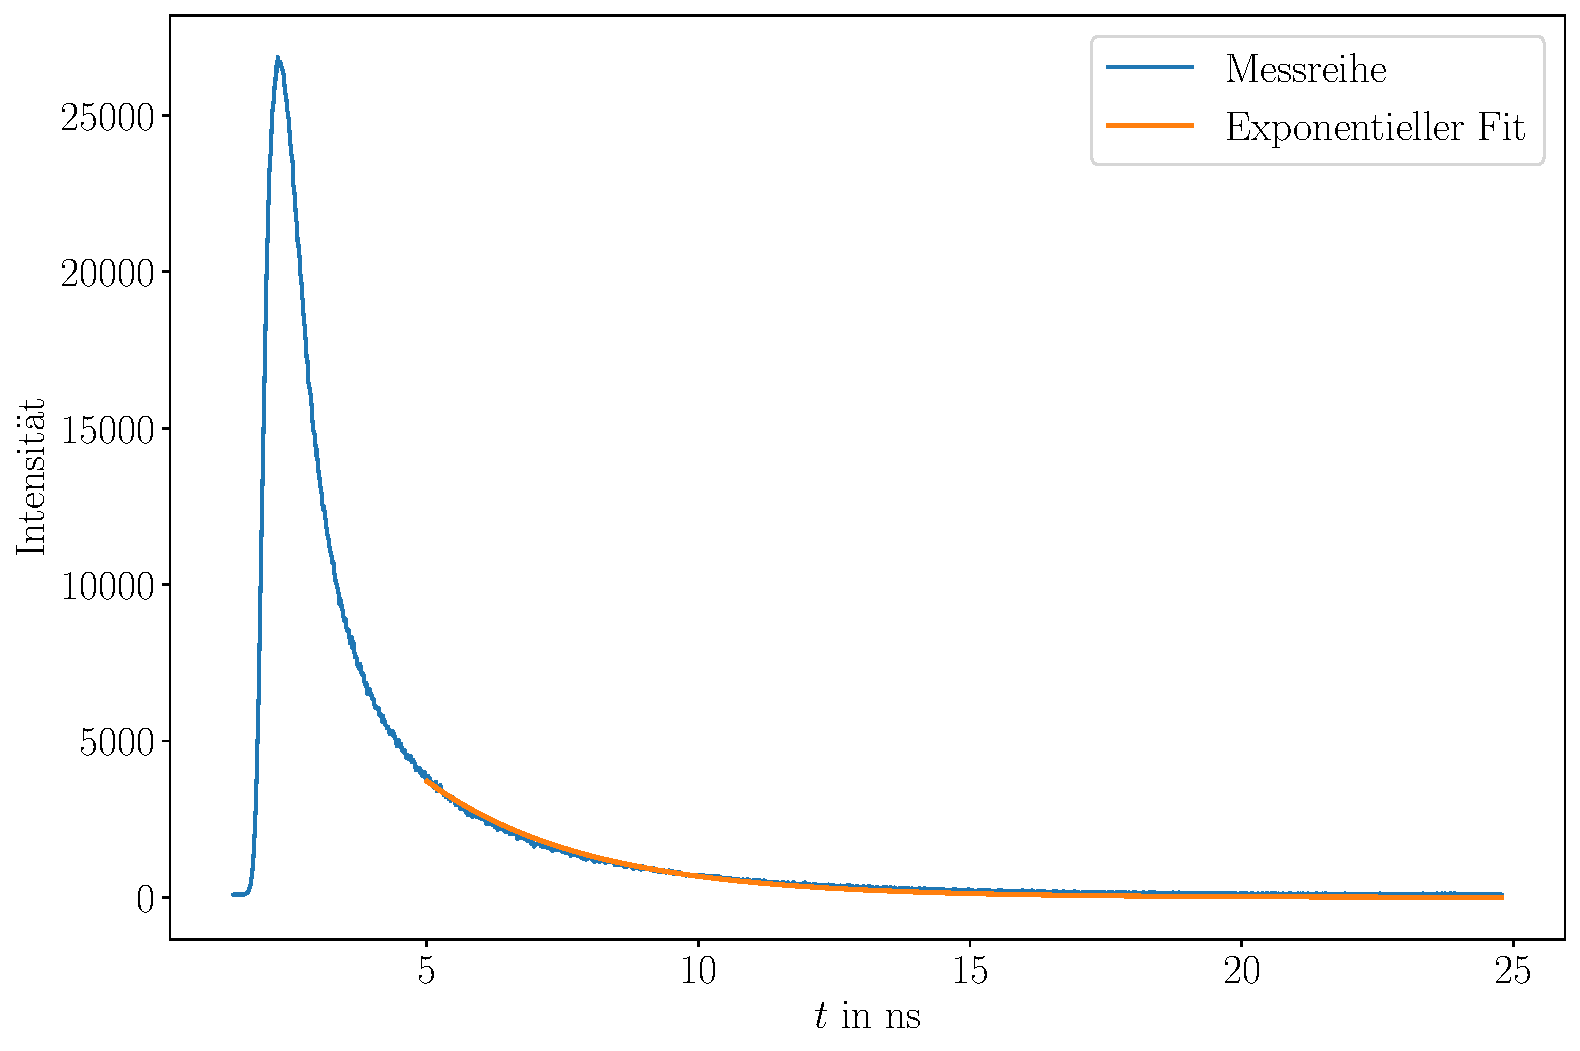
\includegraphics[scale = 0.33, angle = 90]{Lebenszeit/SingleExp/CFP1-c1.pdf}
        &
        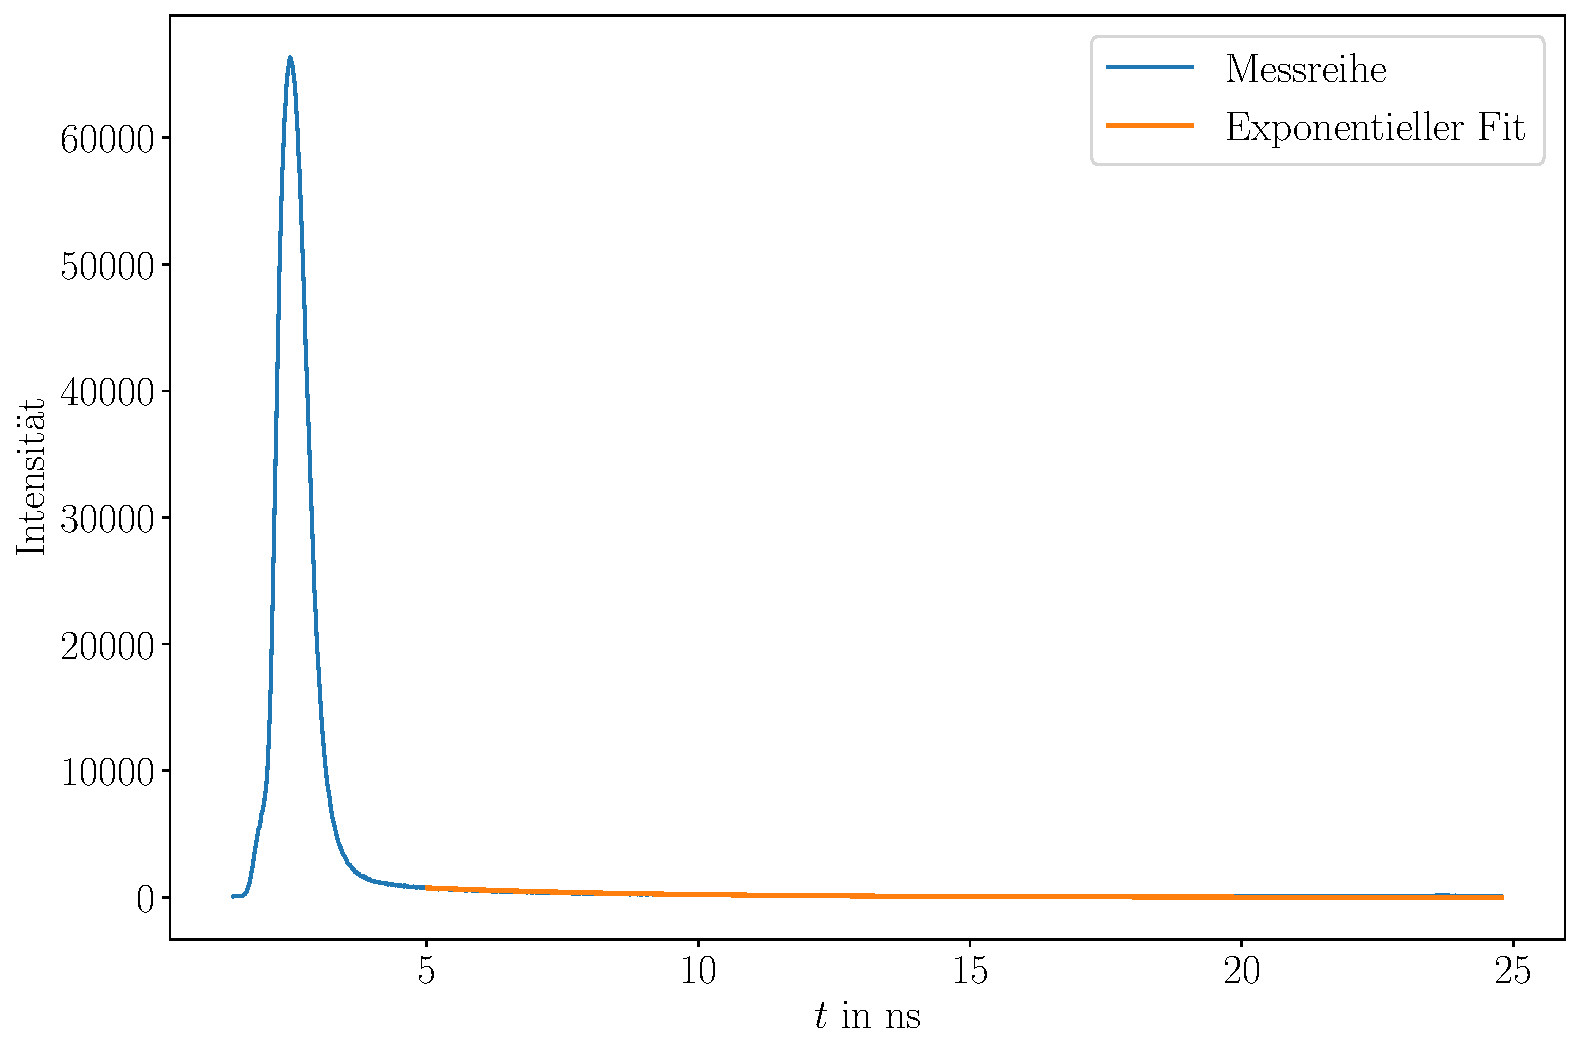
\includegraphics[scale = 0.33, angle = 90]{Lebenszeit/SingleExp/CFP1-c2.pdf}
    \end{tabular}
    \captionof{figure}{CFP1}
    \label{image:singleCFP1}
    \begin{tabular}{c c}
        \textbf{Kanal 1} & \textbf{Kanal 2}\\
        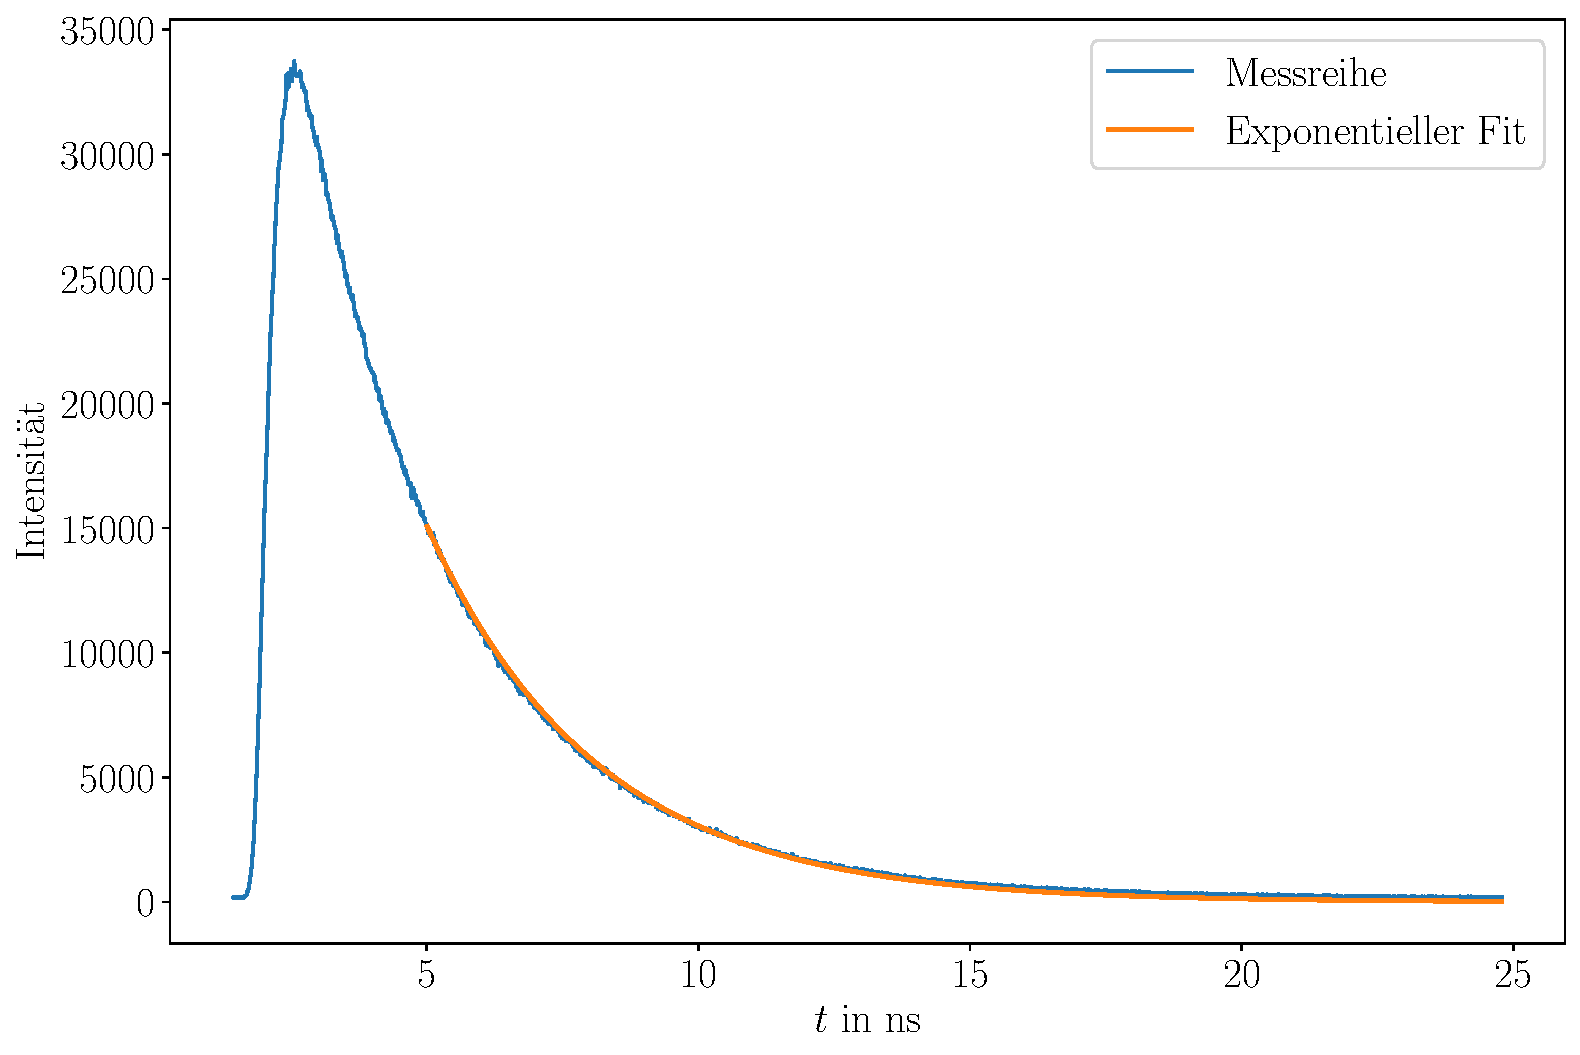
\includegraphics[scale = 0.33, angle = 90]{Lebenszeit/SingleExp/YFP1-c1.pdf}
        &
        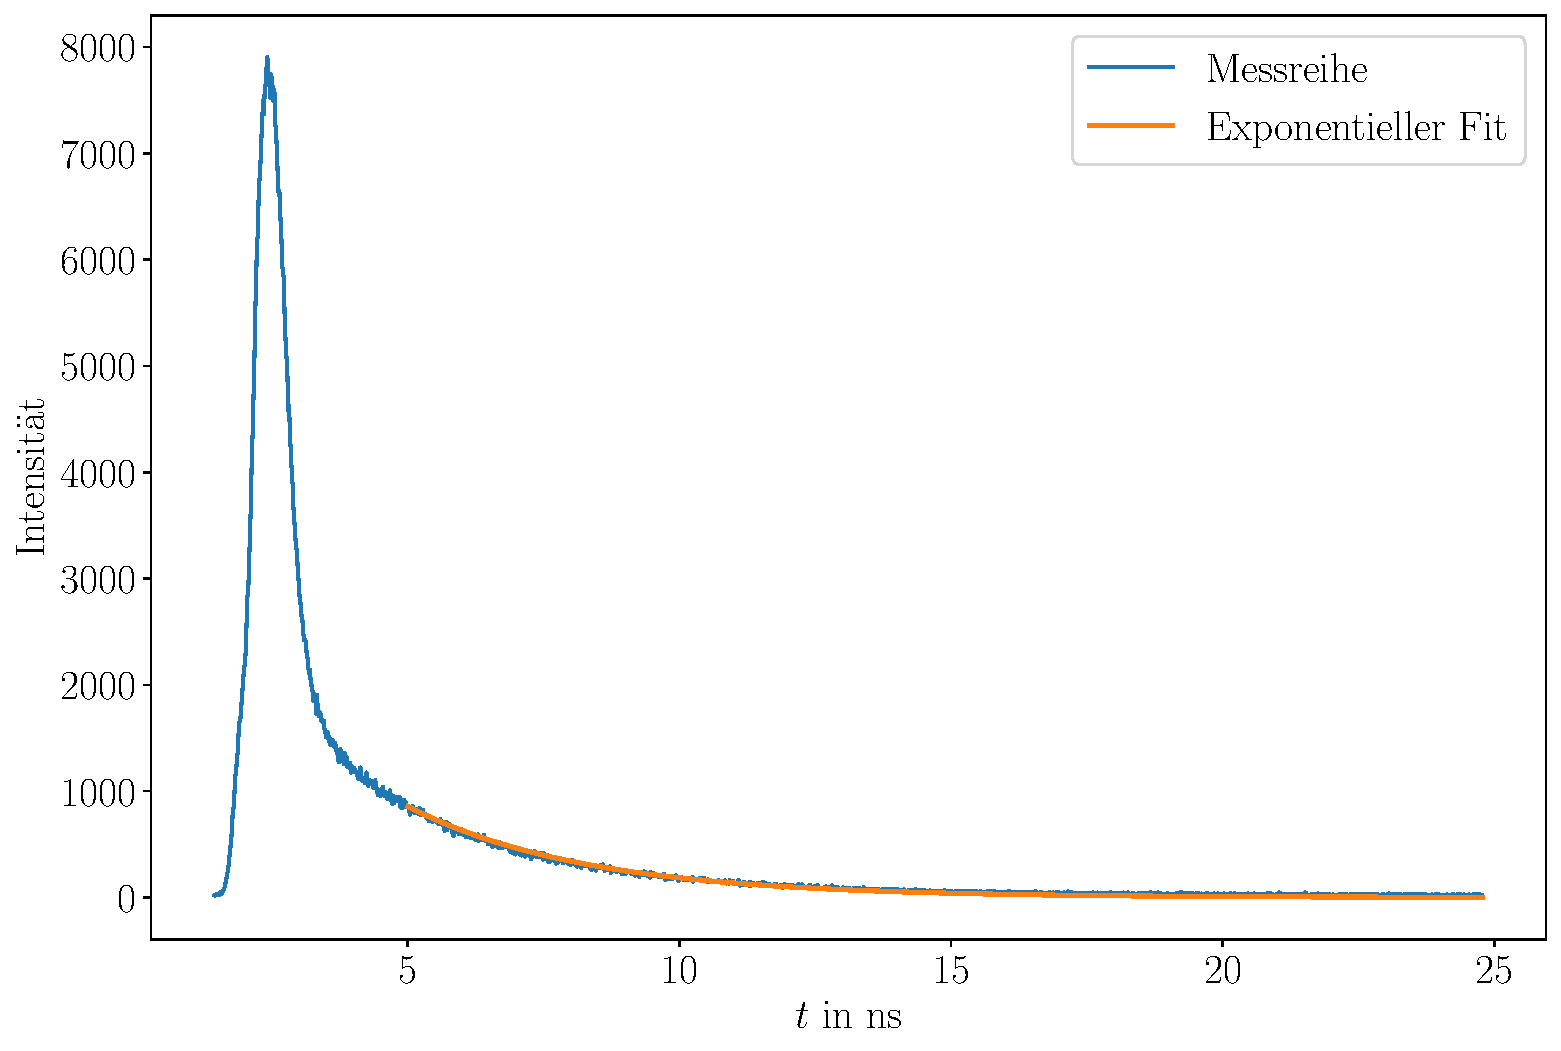
\includegraphics[scale = 0.33, angle = 90]{Lebenszeit/SingleExp/YFP1-c2.pdf}
    \end{tabular}
    \captionof{figure}{YFP1}
    \label{image:singleYFP1}
\end{center}
\newpage
\begin{center}
    \begin{tabular}{c c}
        \textbf{Kanal 1} & \textbf{Kanal 2}\\
        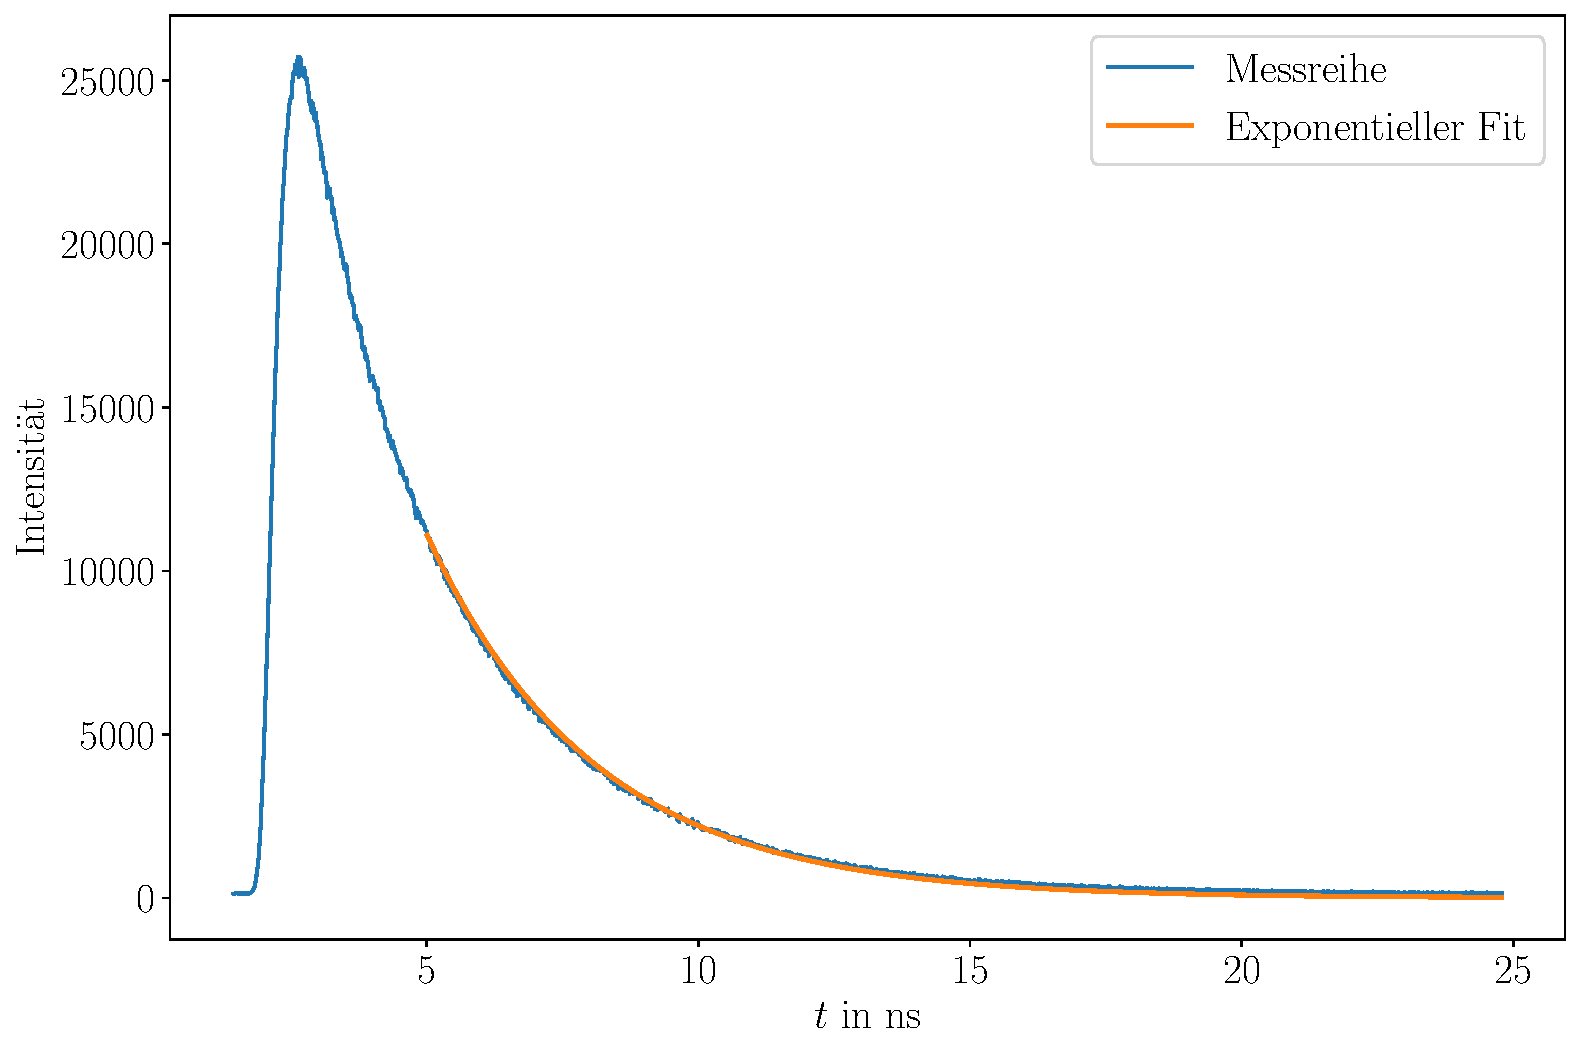
\includegraphics[scale = 0.33, angle = 90]{Lebenszeit/SingleExp/CY1-c1.pdf}
        &
        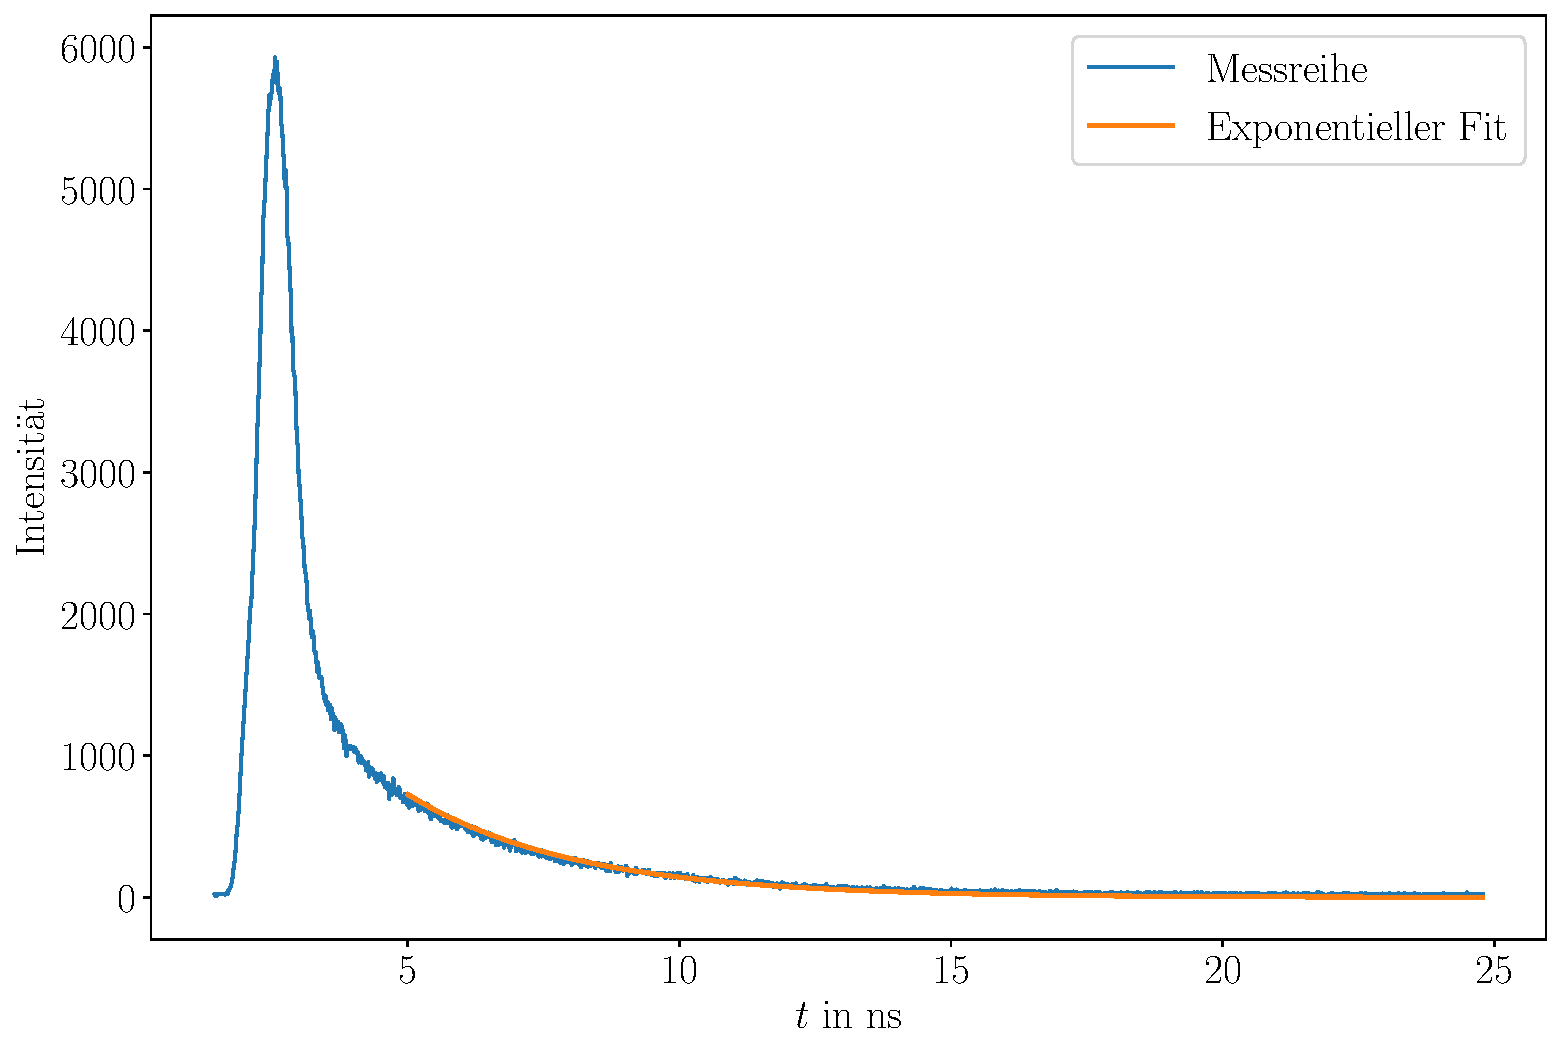
\includegraphics[scale = 0.33, angle = 90]{Lebenszeit/SingleExp/CY1-c2.pdf}
    \end{tabular}
    \captionof{figure}{CY1}
    \label{image:singleCY1}
    \begin{tabular}{c c}
        \textbf{Kanal 1} & \textbf{Kanal 2}\\
        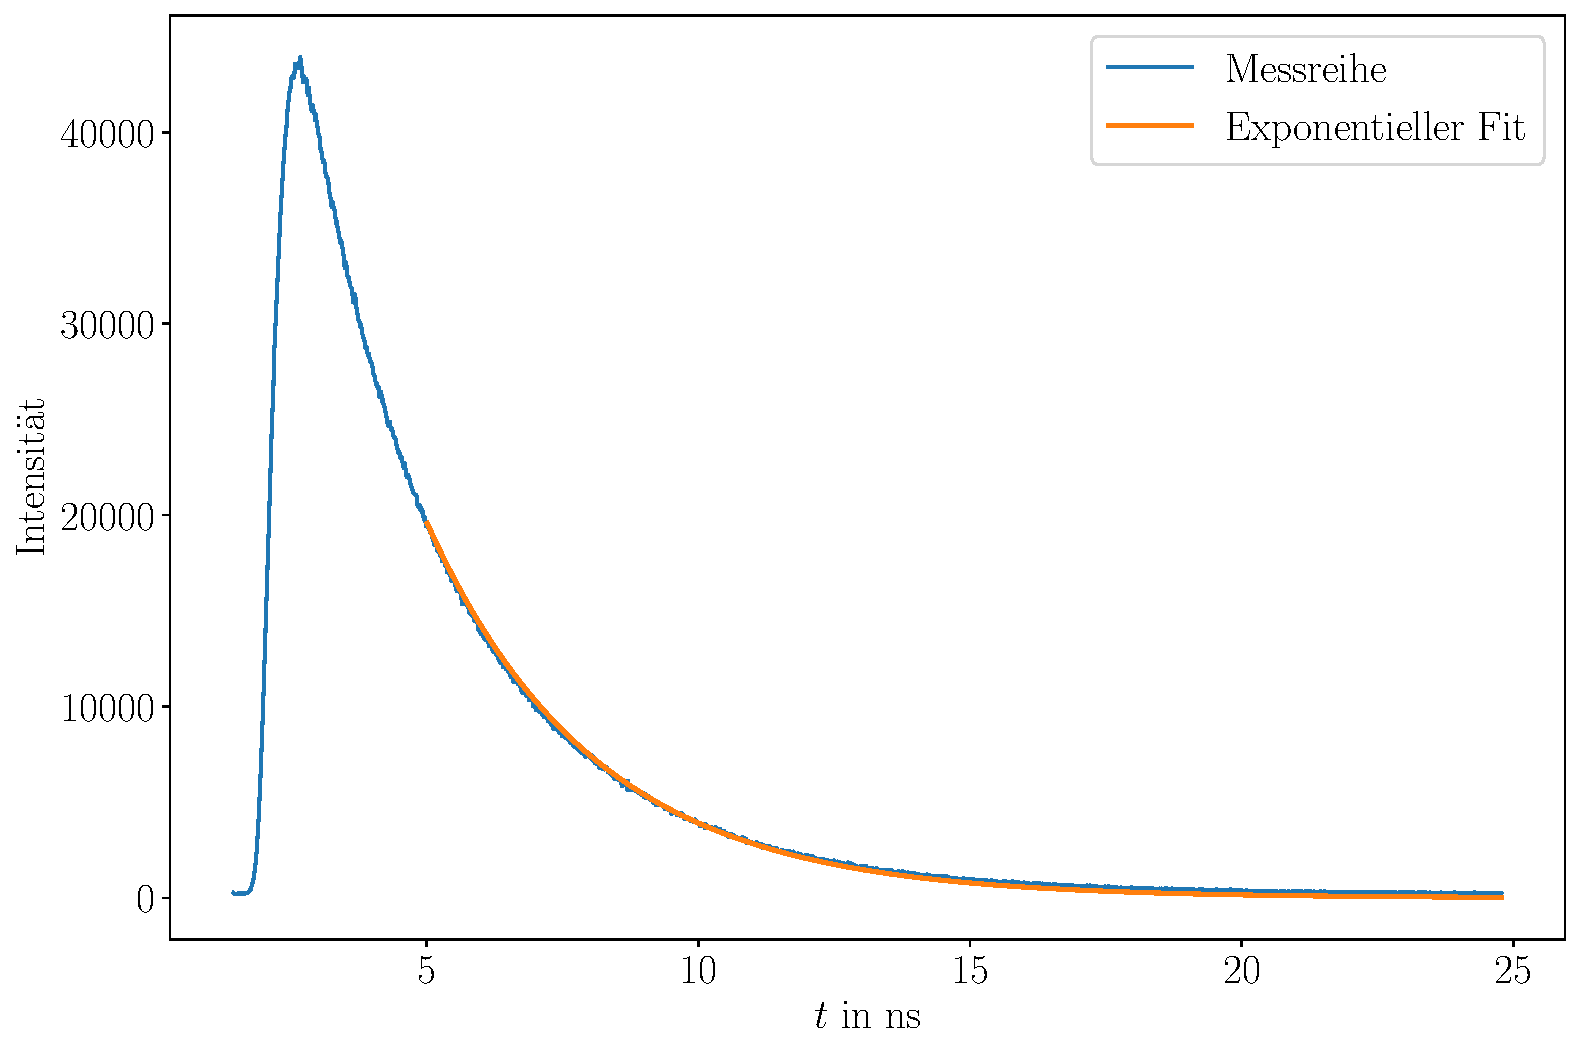
\includegraphics[scale = 0.33, angle = 90]{Lebenszeit/SingleExp/CY3-c1.pdf}
        &
        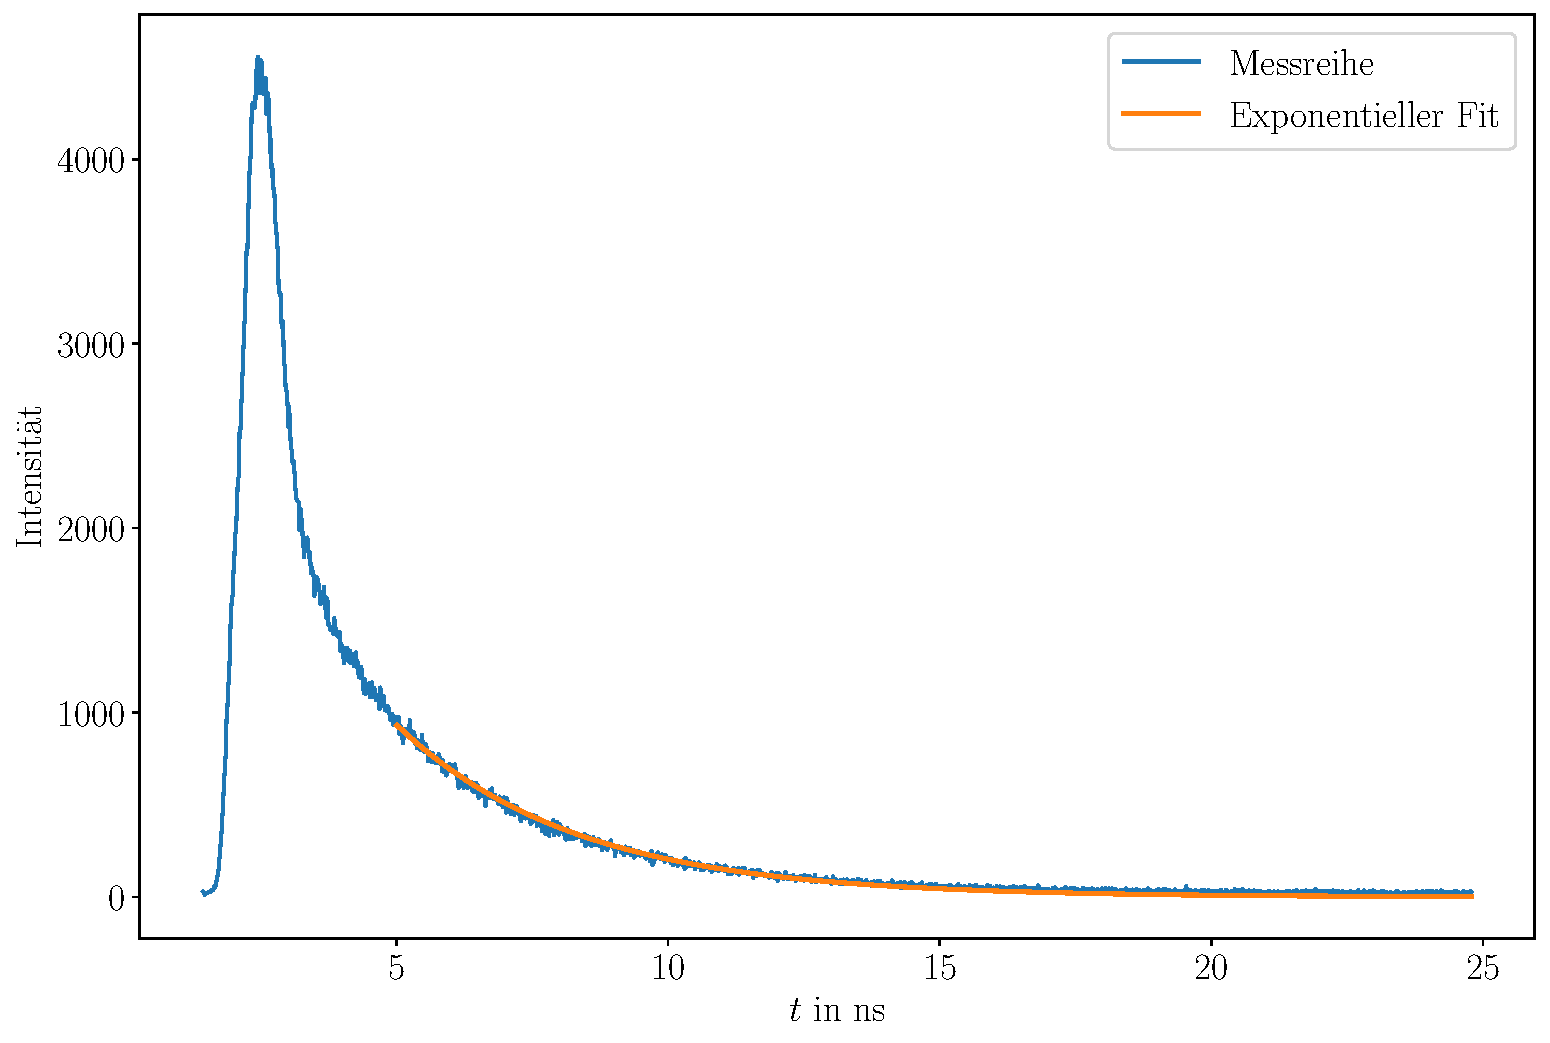
\includegraphics[scale = 0.33, angle = 90]{Lebenszeit/SingleExp/CY3-c2.pdf}
    \end{tabular}
    \captionof{figure}{CY3}
    \label{image:singleCY3}
\end{center}

\paragraph{2)}\textbf{Double-Exponential Fit}\\
Als nächstes wollen wir einen \enquote{Double-Exponential Fit} durch einen ausgewählten Datensatz fitten. Wir haben uns dafür die Probe \textit{CY5} und erneut für eine Anfangszeit $t_{0}=\SI{5}{\nano\metre}$ entschieden. Wichtig ist anzumerken, dass wir für den Fit Kanal 1+2 betrachten. Der Fit hat dann die Form:
\begin{gather}
    N(t) = N_1e^{-\frac{t}{\tau_1}} + N_2e^{-\frac{t}{\tau_2}}
\end{gather}
Da dieser Fit vier Parameter besitzt, $N_1,~N_2,~\tau_1,~\tau_2$, muss die Formel des Fits vereinfacht werden. Dafür klammern wir $N_1$ aus und somit hat der Fit die neue Form:
\begin{gather}
    N(t) = N_1\left[e^{-\frac{t}{\tau_1}} + \frac{N_2}{N_1}e^{-\frac{t}{\tau_2}}\right]
\end{gather}
Für $N_1$ setzen wir die Intensität $N_0$ aus der Tabelle \ref{tab:lebenszeit} für die Probe \textit{CY5} aus Kanal 1. Weiterhin verwenden wir $\frac{N_2}{N_1}$ als \enquote{Guess-Parameter} und verändern diesen zwischen 0 und 30 in kleinen Schritten. Durch diese Veränderung erhalten wir die Lebenszeiten von $\tau_1$ und $\tau_2$ als gefittete Parameter. Um den besten Fit zu finden, berechnen wir $\sum(y_{data}-y_{fit})^2$ und bestimmen davon das Minimum. Der Verlauf von $\sum(y_{data}-y_{fit})^2$ gegen $\frac{N_2}{N_1}$ ist in Abb. \ref{image:doubleOpt} dargestellt und der daraus resultierende Fit in Abb. \ref{image:doubleFit}. Weiterhin wurde in Abb. \ref{image:doubleOptprozess} der generelle Vorgang des Fitprozesses in Abhängigkeit von $\frac{N_2}{N_1}$ visualisiert.
\begin{center}
    \textbf{Ergebnis}\\[0,2cm]
    \begin{tabular}{c c | c c c}
        $\frac{N_2}{N_1}$ & $N_2$ & Min $\sum(y_{data}-y_{fit})^2$ & $\tau_1$ & $\tau_2$ \\
        \hline
        5.51 & 121231 & 0.001224$\cdot10^{10}$ & 4.72 & 2.42 \\
    \end{tabular}
\end{center}
\begin{center}
    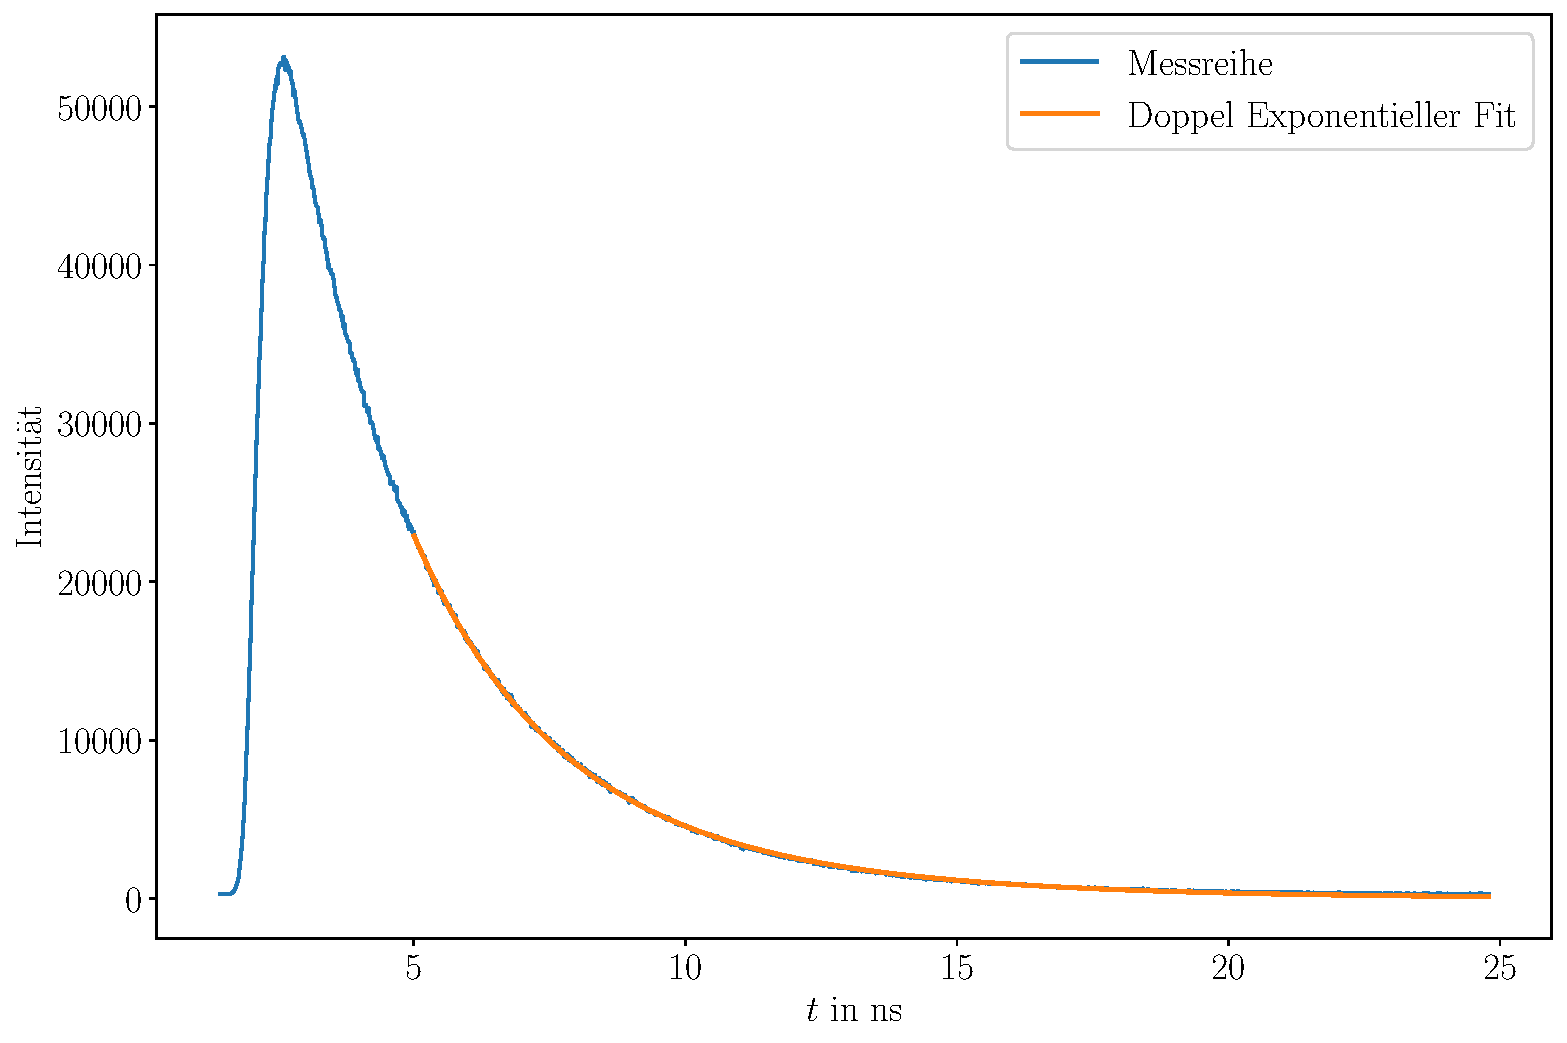
\includegraphics[scale = 0.45]{Lebenszeit/DoubleExp/CY5-c1210.pdf}
    \captionof{figure}{Optimalster Fit}
    \label{image:doubleFit}
\end{center}
\begin{center}
    \includegraphics[scale = 0.45]{Lebenszeit/DoubleExp/Optimize.pdf}
    \captionof{figure}{Optimierung: $\sum(y_{data}-y_{fit})^2$ gegen $\frac{N_2}{N_1}$}
    \label{image:doubleOpt}
\end{center}
\begin{center}
    \begin{tabular}{c c}
        $\frac{N_2}{N_2}=0$ & $\frac{N_2}{N_2}=1.22$\\
        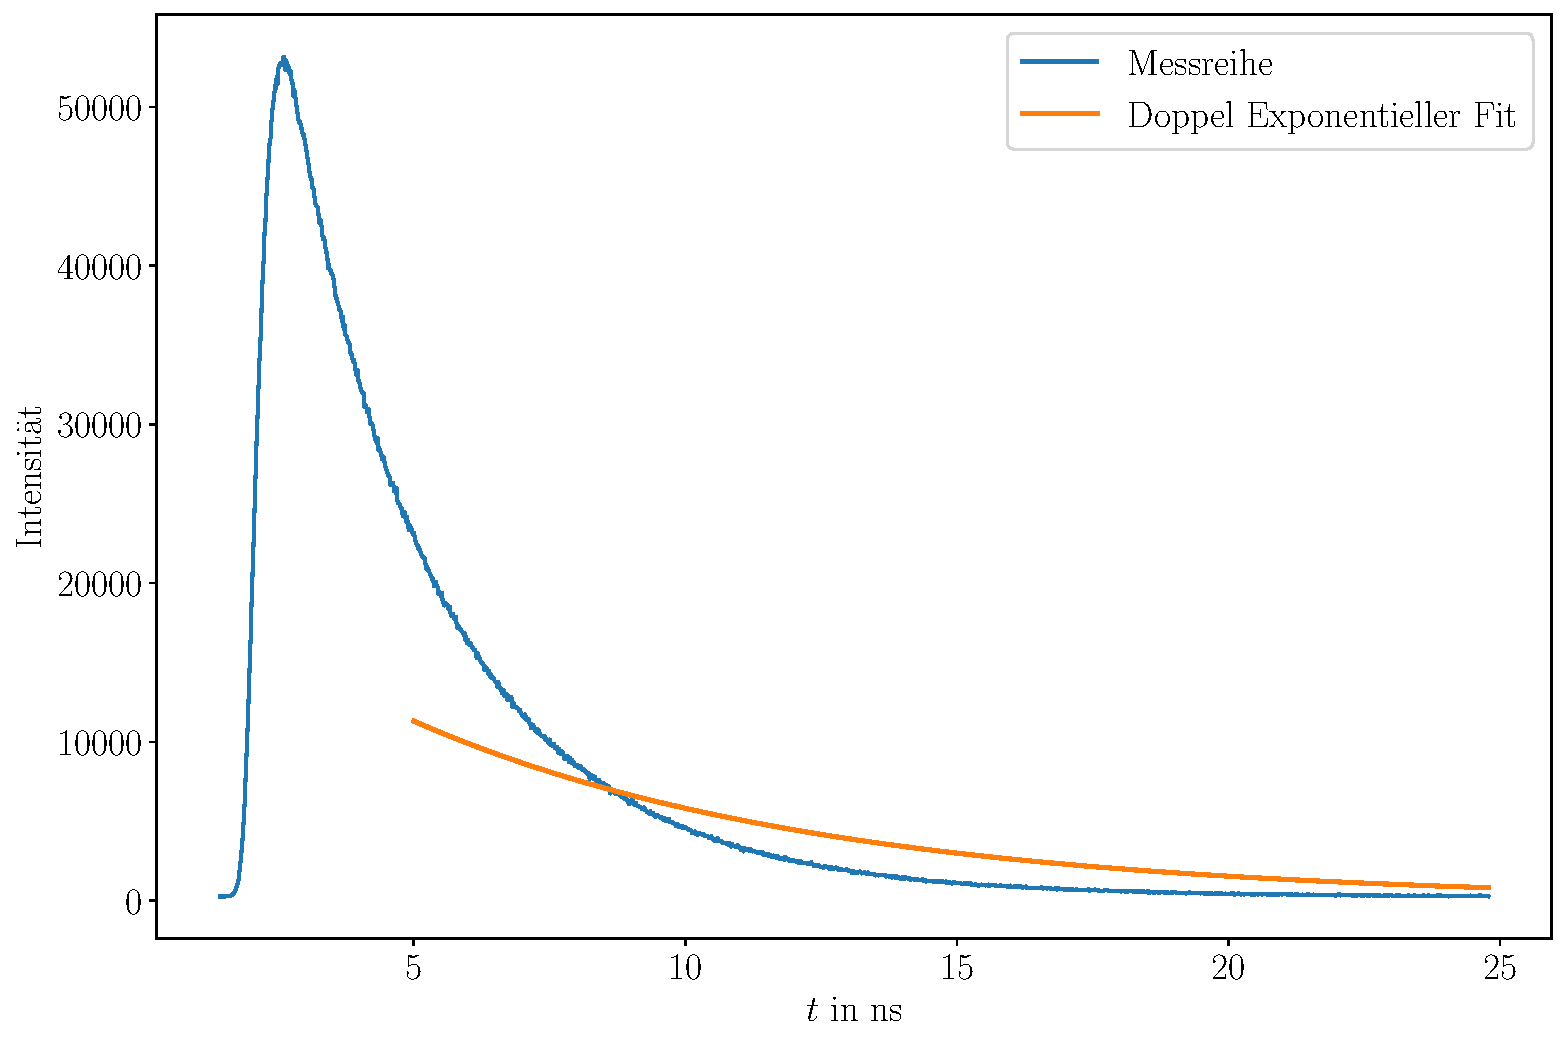
\includegraphics[scale = 0.25]{Lebenszeit/DoubleExp/CY5-c121.pdf}
        &
        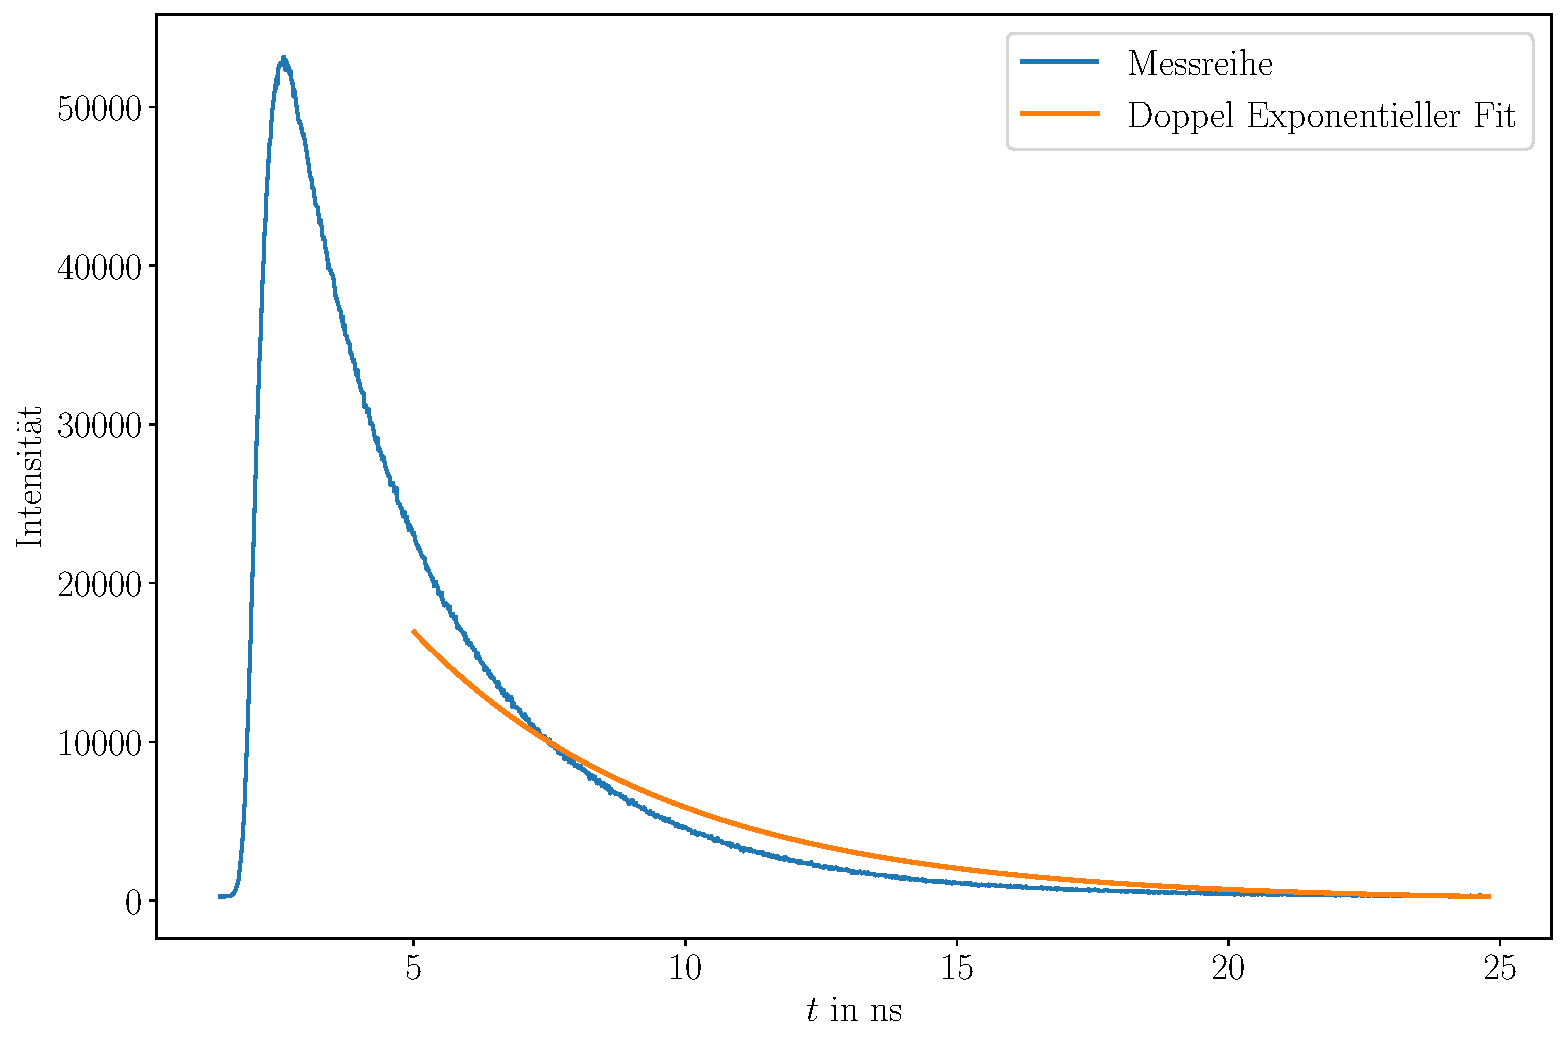
\includegraphics[scale = 0.25]{Lebenszeit/DoubleExp/CY5-c123.pdf}
    \end{tabular}
    \begin{tabular}{c c}
        $\frac{N_2}{N_2}=2.45$ & $\frac{N_2}{N_2}=30$\\
        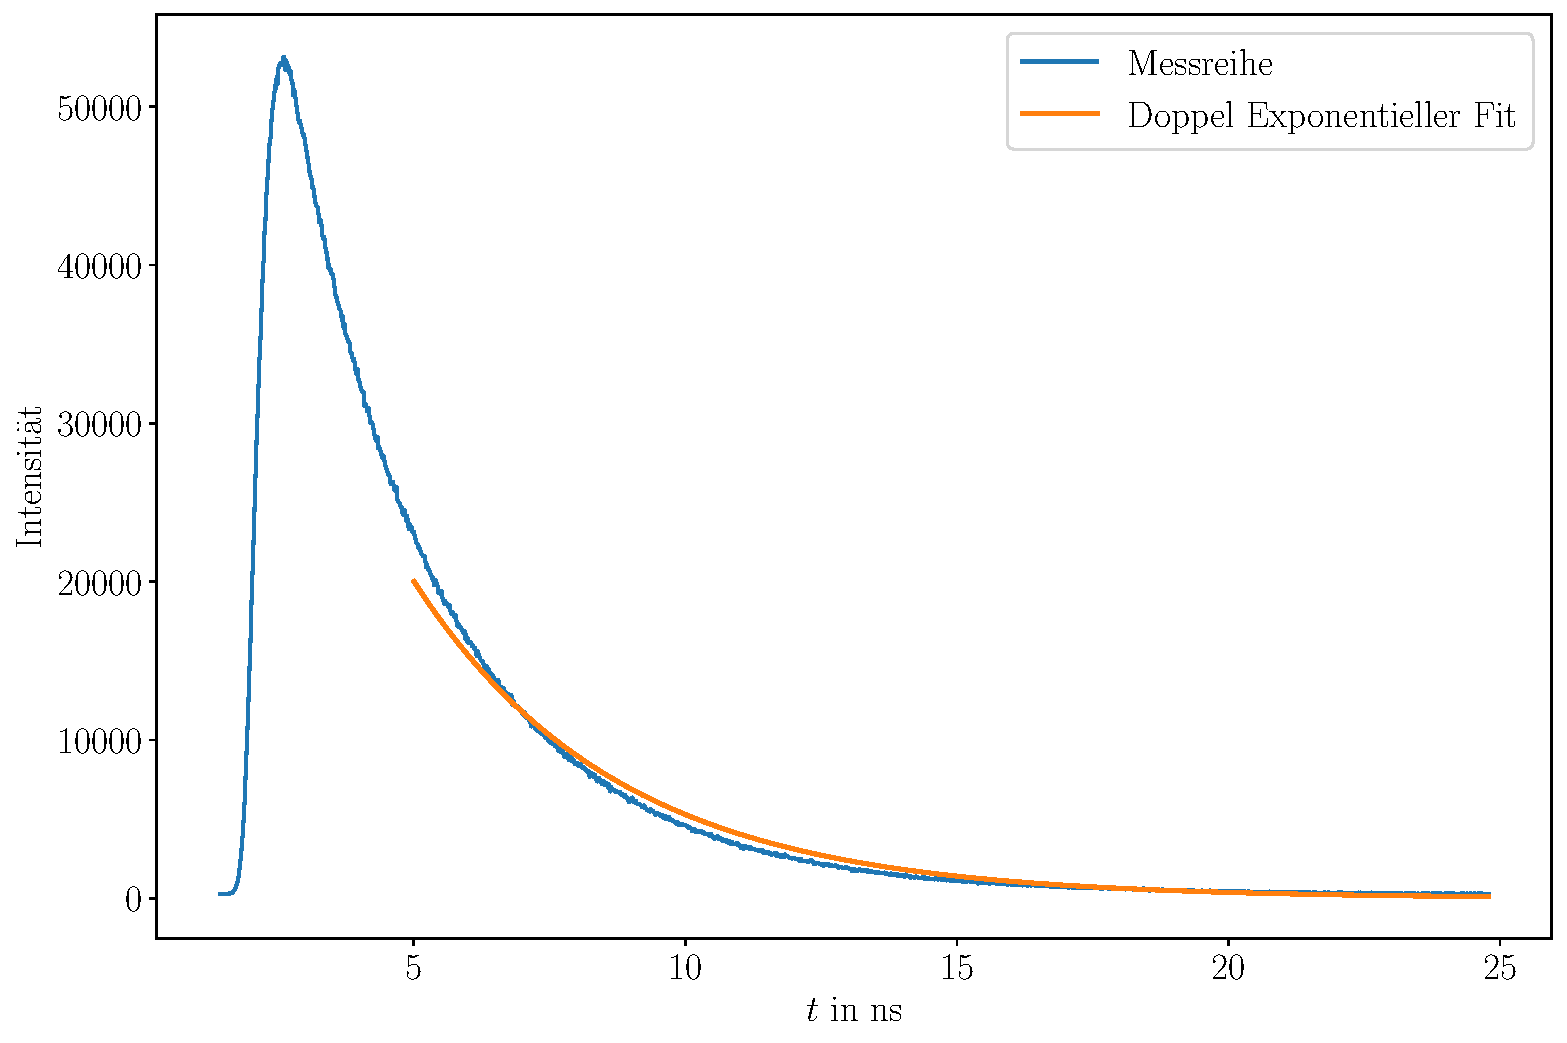
\includegraphics[scale = 0.25]{Lebenszeit/DoubleExp/CY5-c125.pdf}
        &
        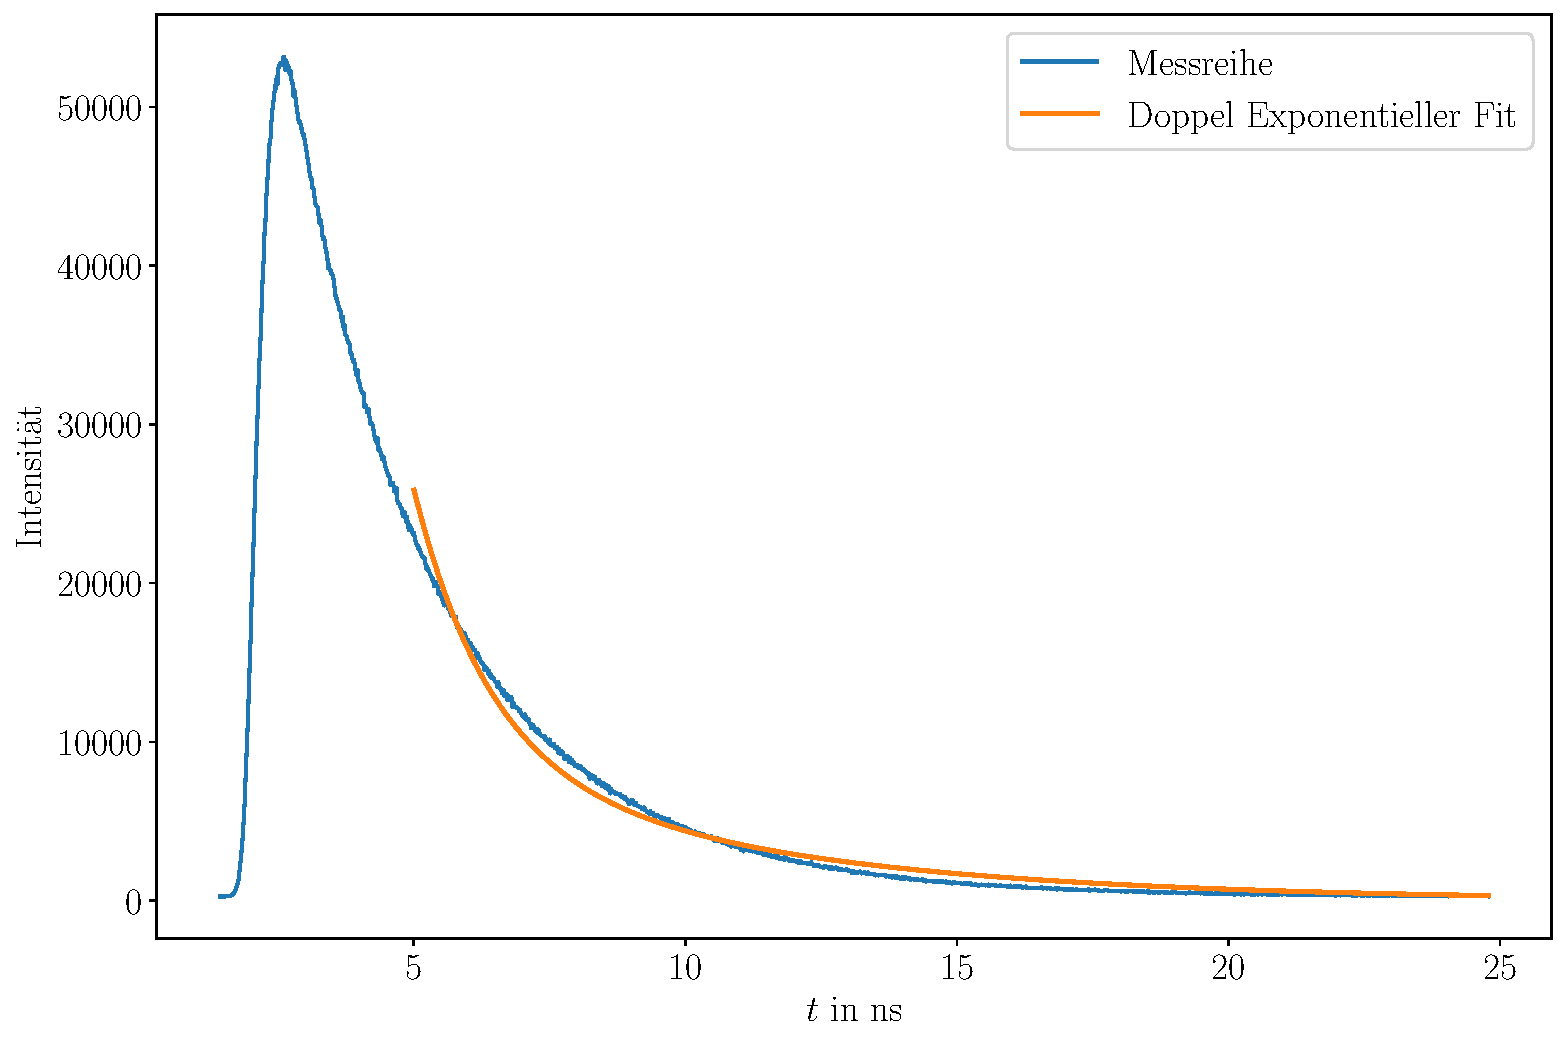
\includegraphics[scale = 0.25]{Lebenszeit/DoubleExp/CY5-c1250.pdf}
    \end{tabular}
    \captionof{figure}{Einige ausgewählte Fits in Abhängigkeit von $\frac{N_2}{N_1}$}
    \label{image:doubleOptprozess}
\end{center}

\paragraph{3)}\textbf{Convolution (dt. Faltung)}\\
In diesem Abschnitt wollen wir die Faltung von der \enquote{Instrument Response Function} (IRF) und der Funktion:
\begin{gather}
    g(t) = 
    \begin{cases}
        0, & t < t_{tot} \\
        N_0 e^{-\frac{t}{\tau}}, & t \geq t_{tot} \\
    \end{cases}
\end{gather}
Als Totzeit $t_{tot}$ wird die Zeit des Maximums gewählt und als $N_0$ die Intensität bei $t_{tot}$, also $N_0 = N(t_{tot})$. Als Fitparameter wird $\tau$ verwendet. Die Faltung ist dann gegeben durch:
\begin{gather}
    f(t) = \text{IRF} * g(t)
\end{gather}
Als IRF benutzen wir einmal das aufgenommene Signal des IRF, das aufgenommene Signal an einer passenden Stelle gespiegelt und eine gefittete Gauß-Kurve an das IRF (siehe Abb. \ref{image:IRF}). Für die Gauß-Kurve benutzen wir die Formel:
\begin{gather}
    N(t) = A \cdot\exp(-\left(\frac{(t-\mu)}{\sqrt{2}\sigma}\right)^2)
\end{gather}
Für die Parameter erhalten wir dann $A = 24986$, $\mu = 2.20$ und $\sigma = 0.21$.
\begin{center}
    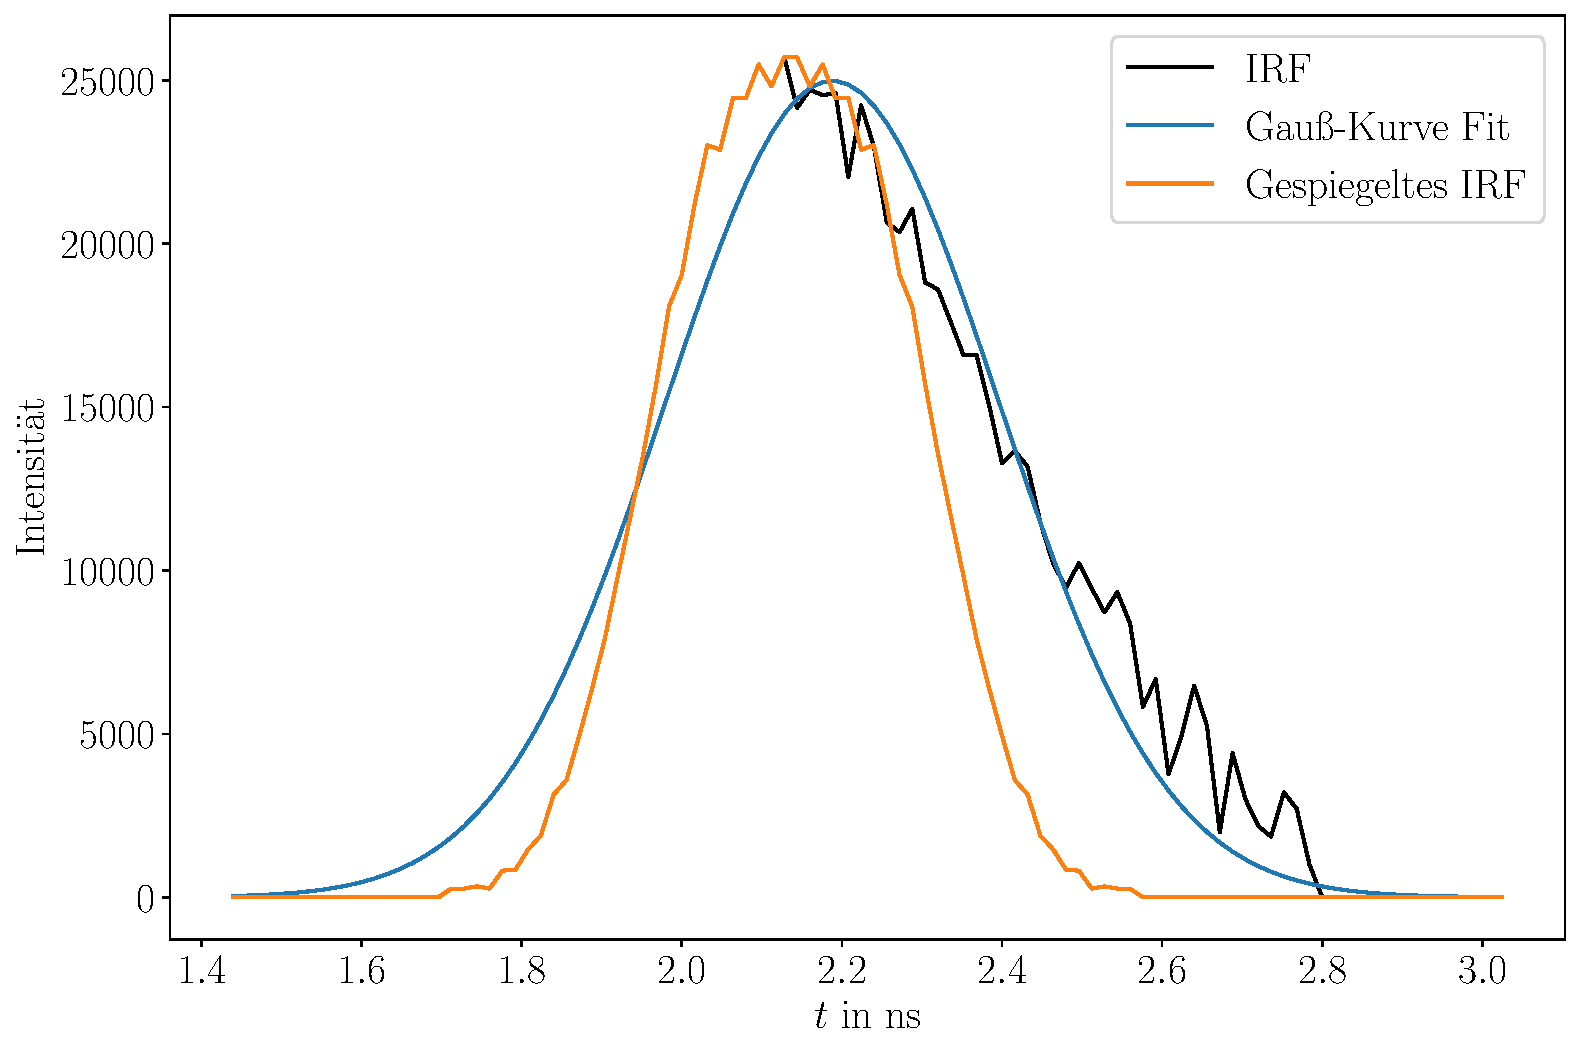
\includegraphics[scale = 0.45]{Lebenszeit/Convolution/IRFfit.pdf}
    \captionof{figure}{Verwendete IRF}
    \label{image:IRF}
\end{center}
\newpage
Für die Faltung verwenden wir das scipy.signal-Module mit der Funktion convolve. Dabei normieren wir die Faltung mit der Summe alle Werte der verwendeten IRF (also $\sum y_{IRF}$). Beim fitten verändern wir nun schrittweise $\tau$ von \SI{2}{\nano\second} bis \SI{5}{\nano\second}. Um den Fit zu optimieren, verwenden wir dieselbe Methode wie in Abschnitt (2) dieses Kapitels und minimieren damit die $\sum(y_{data}-y_{fit})^2$. Die besten Fits sind in Abb. \ref{image:fitIRF} bis \ref{image:fitIRFgauss} mit dem zugehörigen Verlauf von $\sum(y_{data}-y_{fit})^2$ gegen $\tau$.
\begin{center}
    \textbf{Ergebnis}\\[0,2cm]
    \begin{tabular}{c | c c}
        IRF & Min $\sum(y_{data}-y_{fit})^2$ & $\tau$ \\
        \hline
        Aufgenommen & 0.000041$\cdot10^{12}$ & 3.4694 \\
        Gespiegelte & 0.000043$\cdot10^{12}$ & 3.4694 \\
        Gauß-Kurve  & 0.000042$\cdot10^{12}$ & 3.4694 \\
    \end{tabular}
\end{center}
Es ist ersichtlich das alle drei verwendeten Arten von IRF gleichwertig behandelt werden können, da die Werte für $\tau$ bei allen drei Arten von IRF gleich sind. Ein Unterschied könnte ersichtlich werden, wenn man noch kleinere Schritte zwischen \SI{2}{\nano\second} und \SI{5}{\nano\second} macht. Auch ist anzumerken, dass die gefittete Faltung kleiner ist als die tatsächlich gemessene Funktion, was mit der gewählten Normierung zusammenhängen könnte.
\begin{center}
    \begin{tabular}{c c}
        \includegraphics[scale = 0.35, angle = 90]{Lebenszeit/Convolution/IRF/Optimize.pdf}
        &
        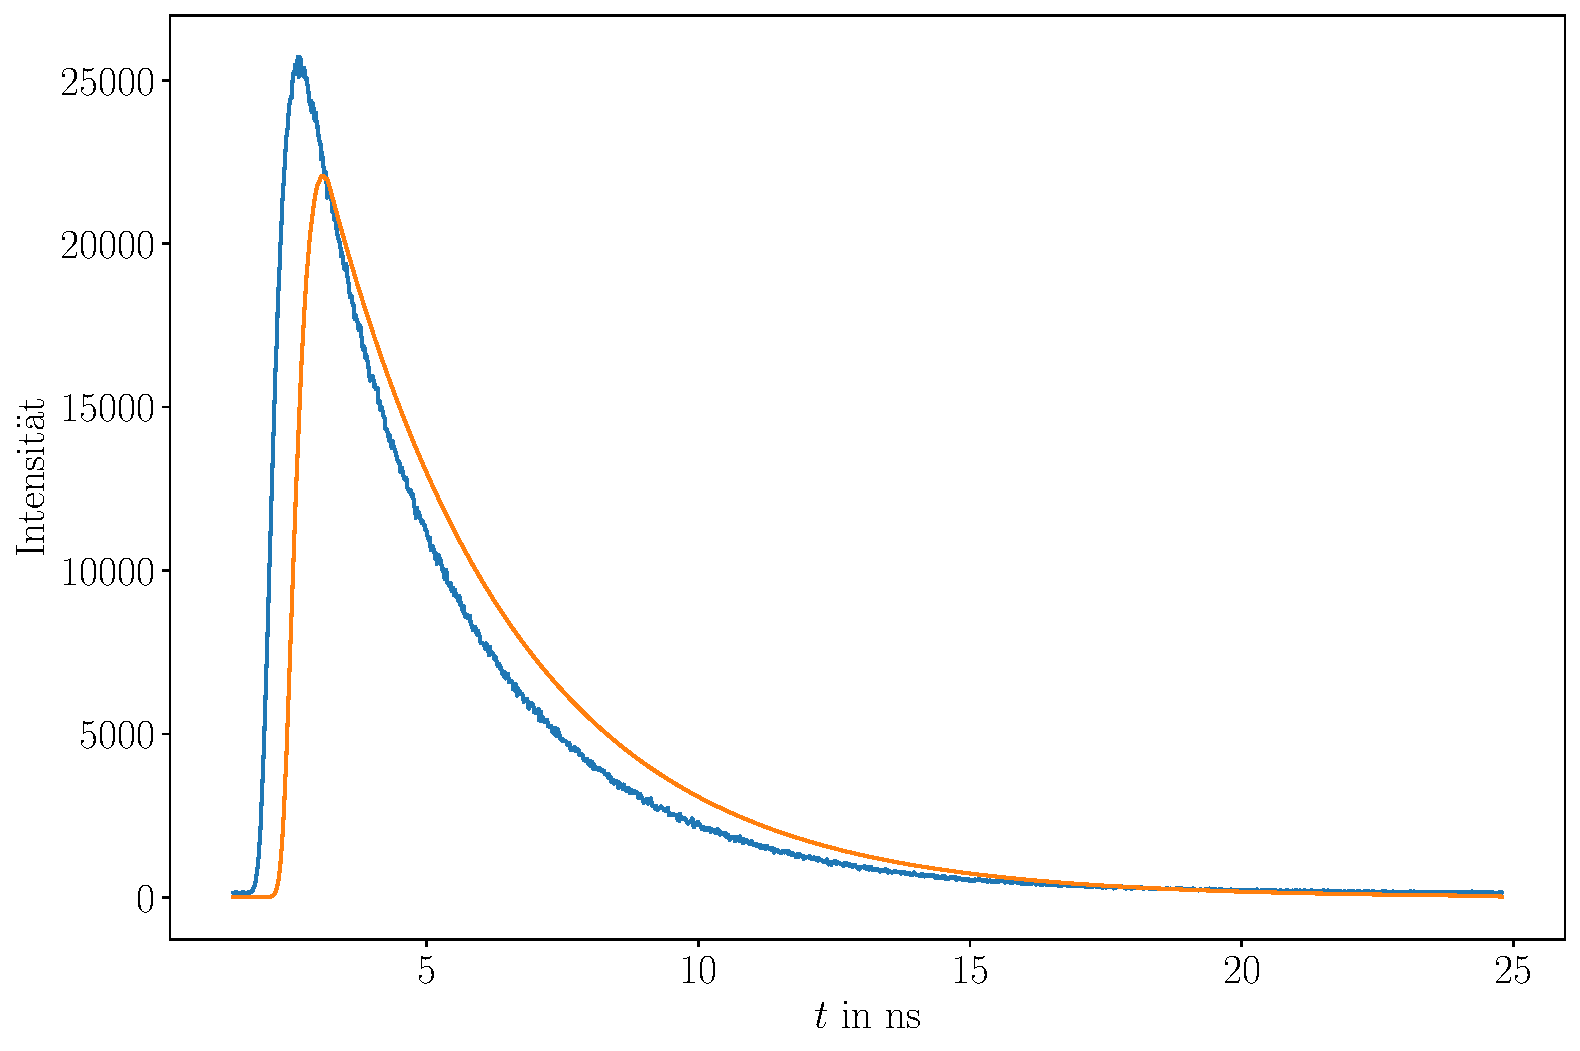
\includegraphics[scale = 0.35, angle = 90]{Lebenszeit/Convolution/IRF/IRF25.pdf}
    \end{tabular}
    \captionof{figure}{Fit für aufgenommenes IRF}
    \label{image:fitIRF}
    \begin{tabular}{c c}
        \includegraphics[scale = 0.35, angle = 90]{Lebenszeit/Convolution/Mirror/Optimize.pdf}
        &
        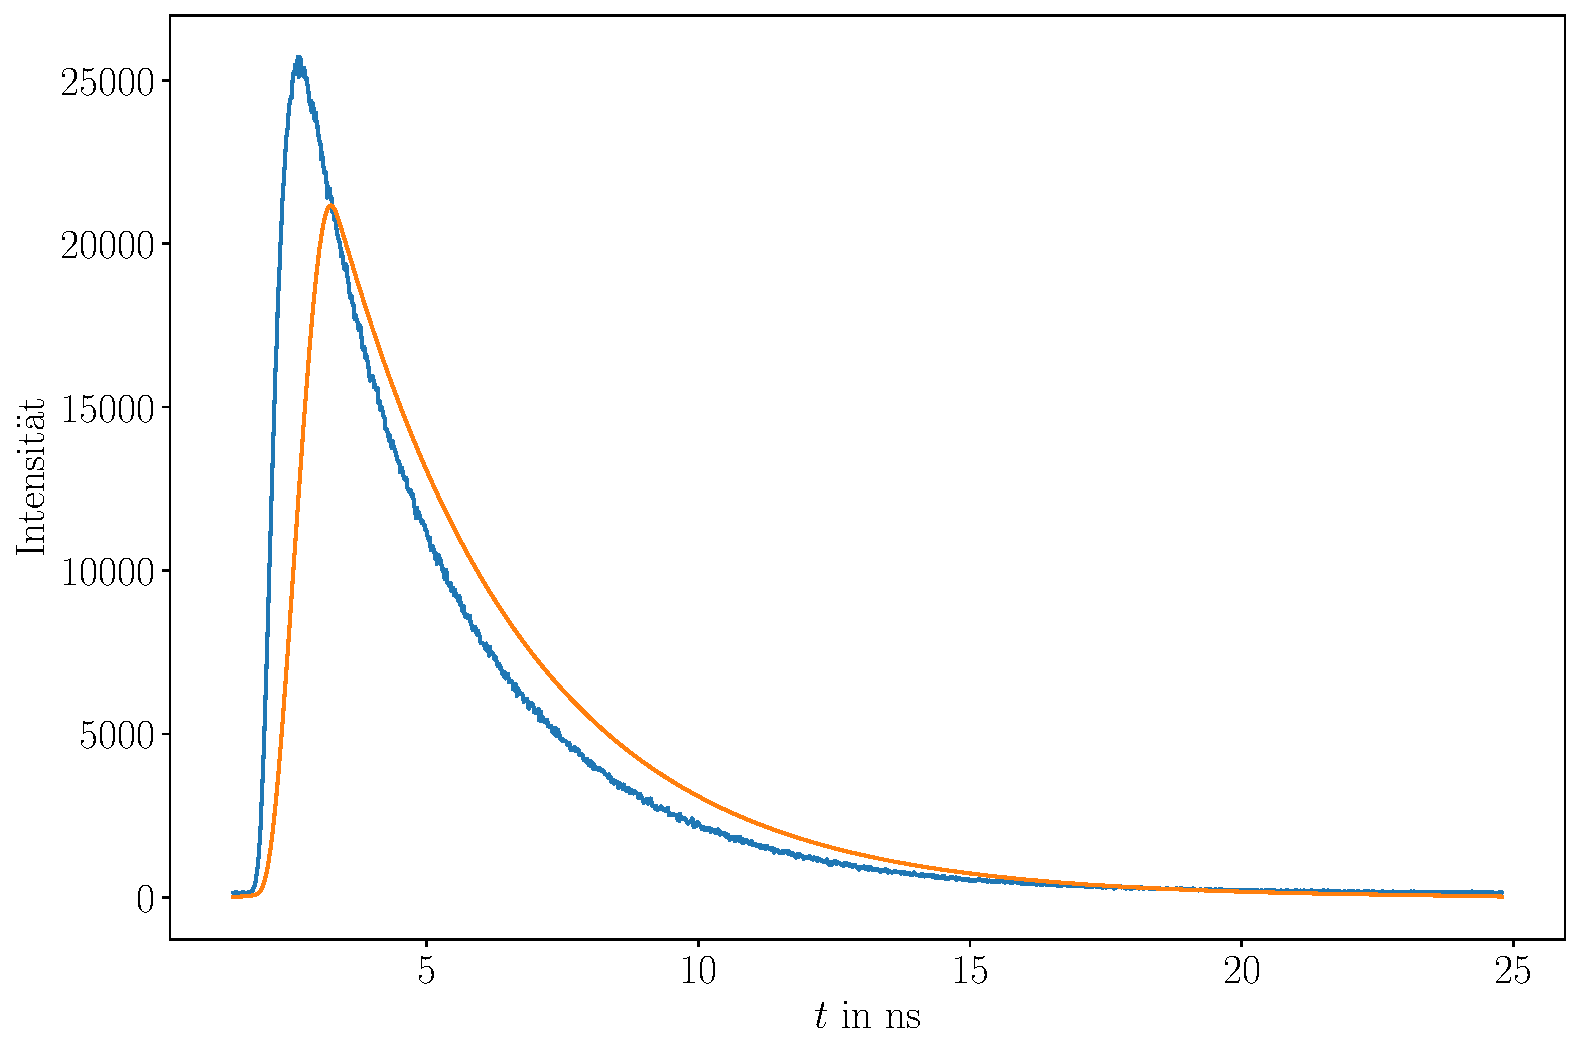
\includegraphics[scale = 0.35, angle = 90]{Lebenszeit/Convolution/Mirror/Mirror25.pdf}
    \end{tabular}
    \captionof{figure}{Fit für gespiegeltes IRF}
    \label{image:fitIRFmir}
    \begin{tabular}{c c}
        \includegraphics[scale = 0.35, angle = 90]{Lebenszeit/Convolution/Gauss/Optimize.pdf}
        &
        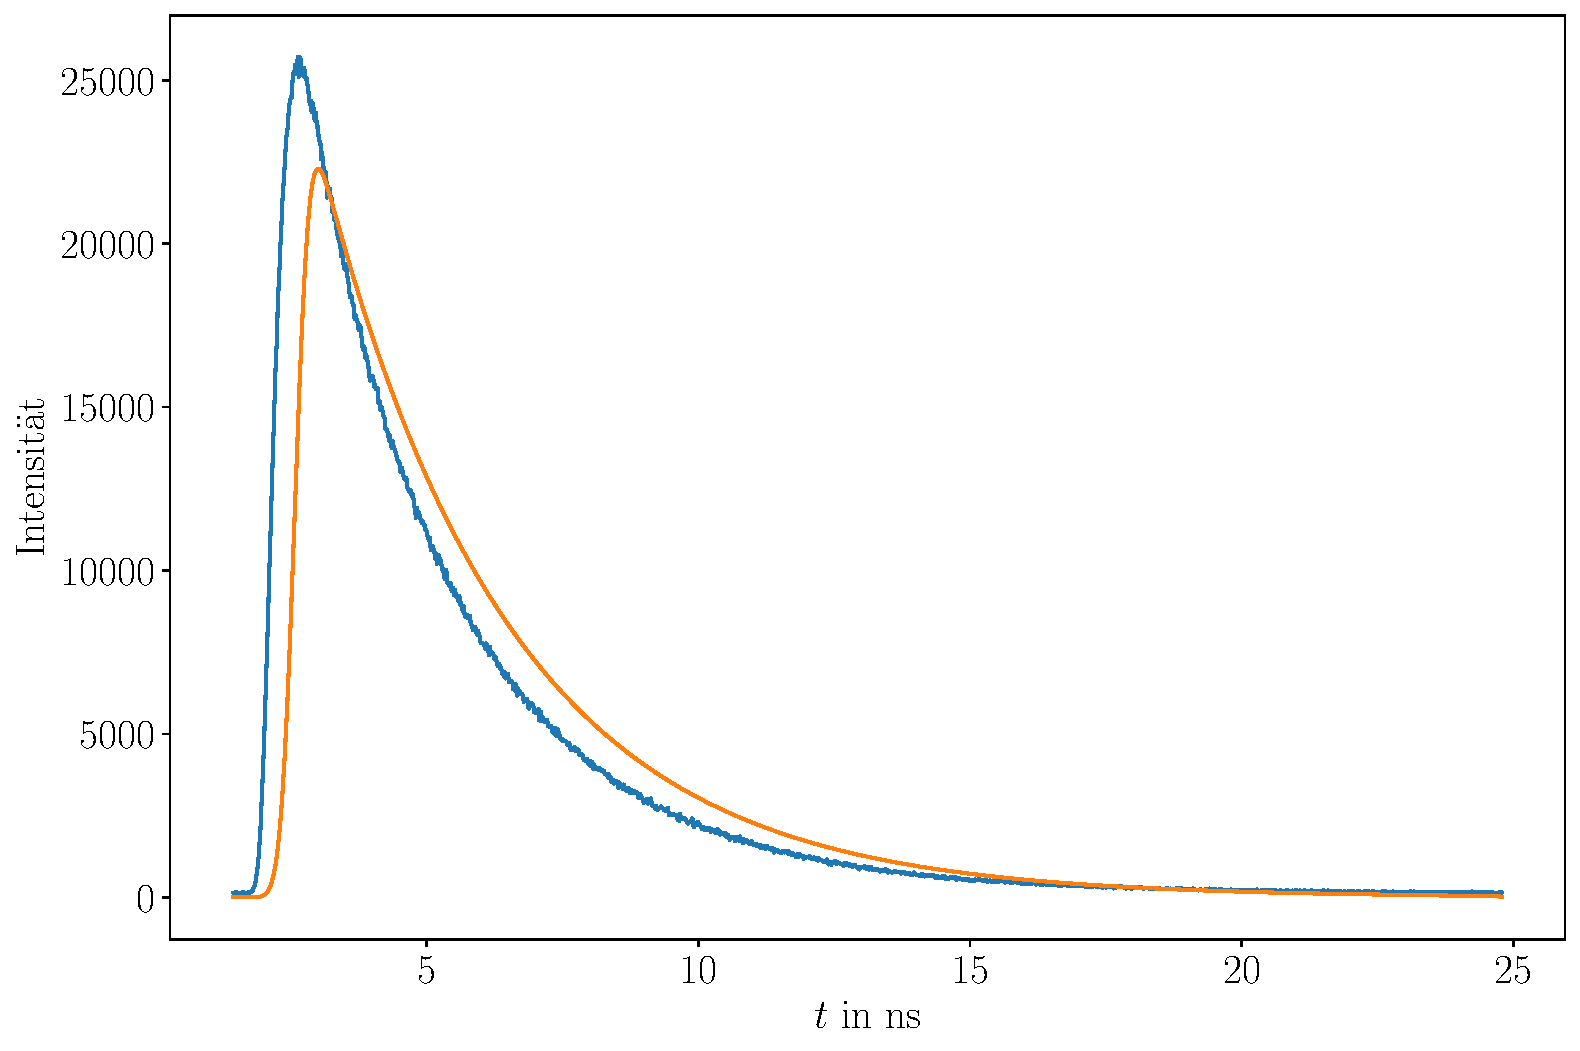
\includegraphics[scale = 0.35, angle = 90]{Lebenszeit/Convolution/Gauss/Gauss25.pdf}
    \end{tabular}
    \captionof{figure}{Fit für Gauß-Kurve}
    \label{image:fitIRFgauss}
\end{center}

\paragraph{4)}\textbf{FRET-Effizienz}\\
Die FRET-Effizienz berechnet sich aus den berechneten Daten wie folgt:
\begin{gather}
    E = 1 - \frac{\tau_{C, Donor}}{\tau_{CY, Donor}}
\end{gather}
Dafür verwenden wir die Mittelwerte aus Tabelle \ref{tab:lebenszeit} für CFP und CY von Kanal 1 und erhalten eine Effizienz  $E = 0,07$.

%\begin{center}
%    \begin{tabular}{c | c c c}
%        $\frac{N_2}{N_1}$ & $\sum(\Delta y)^2$ &  $\tau_1$/nm & $\tau_2$/nm \\
%        \hline
%         0.00 &  0.870933 &  7.52 &  1.00 \\
%         0.61 &  0.414989 &  5.64 &  5.64 \\
%         1.22 &  0.203031 &  4.72 &  4.72 \\
%         1.84 &  0.096182 &  4.15 &  4.15 \\
%         2.45 &  0.041549 &  3.76 &  3.76 \\
%         3.06 &  0.015355 &  3.47 &  3.47 \\
%         3.67 &  0.005649 &  3.25 &  3.25 \\
%         4.29 &  0.002986 &  4.23 &  2.78 \\
%         4.90 &  0.001636 &  4.53 &  2.57 \\
%         5.51 &  0.001224 &  4.72 &  2.42 \\
%         6.12 &  0.001440 &  4.85 &  2.30 \\
%         6.73 &  0.002082 &  4.96 &  2.21 \\
%         7.35 &  0.003012 &  5.04 &  2.13 \\
%         7.96 &  0.004141 &  5.12 &  2.06 \\
%         8.57 &  0.005403 &  5.18 &  2.00 \\
%         9.18 &  0.006756 &  5.23 &  1.95 \\
%         9.80 &  0.008168 &  5.28 &  1.90 \\
%        10.41 &  0.009615 &  5.32 &  1.86 \\
%        11.02 &  0.011083 &  5.36 &  1.83 \\
%        11.63 &  0.012557 &  5.39 &  1.79 \\
%        12.24 &  0.014030 &  5.43 &  1.76 \\
%        12.86 &  0.015496 &  5.46 &  1.73 \\
%        13.47 &  0.016948 &  5.48 &  1.71 \\
%        14.08 &  0.018385 &  5.51 &  1.68 \\
%        14.69 &  0.019803 &  5.53 &  1.66 \\
%        15.31 &  0.021200 &  5.55 &  1.64 \\
%        15.92 &  0.022576 &  5.57 &  1.62 \\
%        16.53 &  0.023929 &  5.59 &  1.60 \\
%        17.14 &  0.025260 &  5.61 &  1.59 \\
%        17.76 &  0.026567 &  5.63 &  1.57 \\
%        18.37 &  0.027851 &  5.64 &  1.55 \\
%        18.98 &  0.029113 &  5.66 &  1.54 \\
%        19.59 &  0.030352 &  5.67 &  1.52 \\
%        20.20 &  0.031568 &  5.68 &  1.51 \\
%        20.82 &  0.032762 &  5.70 &  1.50 \\
%        21.43 &  0.033935 &  5.71 &  1.49 \\
%        22.04 &  0.035087 &  5.72 &  1.47 \\
%        22.65 &  0.036218 &  5.73 &  1.46 \\
%        23.27 &  0.037329 &  5.75 &  1.45 \\
%        23.88 &  0.038421 &  5.76 &  1.44 \\
%        24.49 &  0.039493 &  5.77 &  1.43 \\
%        %25.10 &  0.040547 &  5.78 &  1.42 \\
%        %25.71 &  0.041582 &  5.79 &  1.41 \\
%        %26.33 &  0.042600 &  5.79 &  1.41 \\
%        %26.94 &  0.043601 &  5.80 &  1.40 \\
%        %27.55 &  0.044586 &  5.81 &  1.39 \\
%        %28.16 &  0.045554 &  5.82 &  1.38 \\
%        %28.78 &  0.046506 &  5.83 &  1.37 \\
%        %29.39 &  0.047443 &  5.84 &  1.37 \\
%        %30.00 &  0.048365 &  5.84 &  1.36 \\
%    \end{tabular}
%\end{center}